%---------------------------------------------------------------------
\chapter{Implementation}
%---------------------------------------------------------------------

This chapter describes how the design of Chapter~4 was built: the technology stack, the preparation
of the reference data and the retrieval index, the agent loop, the tools, the prompts, the guardrails
and loop bounds, the user interface and the repository structure. Together with
Appendix~\ref{app:run}, it is intended to allow another student to reproduce the system.

\section{Technology Stack}

Table~\ref{tab:stack} lists the technologies used, with the exact versions installed in the project's
virtual environment.

\begin{table}[H]
\centering
\caption{Technology stack}
\label{tab:stack}
\small
\begin{tabularx}{\linewidth}{@{}>{\raggedright\arraybackslash}p{3.4cm} >{\raggedright\arraybackslash}p{4.4cm} >{\raggedright\arraybackslash}X@{}}
\toprule
\textbf{Layer} & \textbf{Choice (version)} & \textbf{Reason} \\ \midrule
Language & Python 3.13.7 & Standard for agent tooling \\
Orchestration & LangGraph 1.2.20~\cite{langgraph} & Explicit state graph with conditional edges and reducers \\
Schemas & Pydantic 2.14.3~\cite{pydantic} & Typed tool inputs and outputs, validated at run time \\
Language model (optional) & Llama~3.1~8B Instant~\cite{llama3} via Groq API, client 1.7.0~\cite{groq} & Small, fast model with JSON output; free tier \\
Retrieval & BM25~\cite{robertson2009bm25}, implemented in Python & Transparent keyword ranking over a small official corpus \\
OCR (optional) & EasyOCR~\cite{easyocr} & Label images; not installed for the reported runs \\
Persistence & SQLite~\cite{sqlite} (Python \texttt{sqlite3}) & Checkpoints, review queue, decisions, case history \\
Interface & Streamlit 1.67.0~\cite{streamlit} with custom HTML and CSS & Web pages for requesters and reviewers \\
Tables & pandas 3.1.1 & Reviewer and evaluation tables \\
\bottomrule
\end{tabularx}
\end{table}

The design document proposed Chroma with \texttt{bge-small} embeddings as the vector store. This was
replaced by BM25 because the corpus contains only 21 short passages whose relevant terms (district
names, materials, product names) are exact keywords, for which lexical matching is reliable, and
because BM25 needs no model download, so the evaluation runs offline and deterministically. Dense
retrieval would become preferable if the full scanned GI applications were indexed (Section~10.2).

\section{Data Preparation and Indexing}

\paragraph{Registry.} Each of the fifteen products is stored as a record with its GI application number
(where known), state, goods class, list of registered districts or places, list of aliases, registered
materials, a \texttt{state\_wide} flag and a source identifier. Aliases were written by the team from
common market names, for example ``kanjivaram'', ``kanjeevaram'' and ``kanchi pattu'' for Kancheepuram
Silk. When several aliases match a label, the longest match is chosen, so that ``Sambalpuri ikat''
resolves to Sambalpuri Bandha rather than to Pochampalli Ikat through the shorter alias ``ikat''.

\paragraph{Census.} The 31 rows of the PIB annexure were transcribed into a table of state, weavers and
allied workers, keyed by state name. The All-India total in the source (26,73,891 weavers) was used to
check the transcription.

\paragraph{Retrieval corpus and index.} The corpus has 21 passages: three for each of the three
original products and one for each of the twelve catalogue products, the latter taken from the
description in the PIB GI catalogue. Each passage carries its product and a page reference as metadata.
Documents are not chunked further, because each passage is a single paragraph of 20 to 59 words that
describes one aspect of one product; splitting would separate district names from the product they
refer to. Text is lower-cased and tokenised into alphabetic words, the product name is appended to
each passage, and BM25 statistics (document frequencies and average length) are computed once at
start-up. Scoring uses the standard parameters $k_1 = 1.5$ and $b = 0.75$:
\begin{equation}
\mathrm{score}(q,d) = \sum_{t \in q} \mathrm{IDF}(t)\,\frac{f(t,d)\,(k_1+1)}{f(t,d) + k_1\left(1 - b + b\,\frac{|d|}{\overline{|d|}}\right)},
\end{equation}
where $f(t,d)$ is the frequency of term $t$ in passage $d$ and
$\mathrm{IDF}(t) = \ln\!\left(1 + \frac{N - n_t + 0.5}{n_t + 0.5}\right)$ for $N$ passages of which
$n_t$ contain $t$. The search returns at most five passages with a score above zero, optionally
restricted to one product. A first-iteration search is considered adequate evidence only if its top
score is at least 2.0. This value was fixed by the team during development as a conservative
minimum and was not tuned on the test set; once the product has been resolved through the registry,
any passage retrieved for that product is accepted as document support.

\paragraph{Simulated producer records.} The generator described in Section~3.4 is run at import time with
a fixed seed, producing identifiers of the form \texttt{WV-KAN-001} for weavers and
\texttt{B-KAN-0010} for batches, where the three-letter code identifies the product.

\section{Core Agent Loop}

Algorithm~\ref{alg:loop} gives the agent loop in pseudocode.

\begin{algorithm}[H]
\caption{LoomTrace agent loop}
\label{alg:loop}
\begin{algorithmic}[1]
\Require claim text $x$, maximum iterations $L = 3$
\State $f \gets \textsc{Extract}(x)$; \quad $i \gets 0$; \quad $E \gets [\,]$
\Loop
  \State $(P, q, \mathit{resolve}) \gets \textsc{Plan}(f, i)$ \Comment{checks, query, alias flag}
  \State $E \gets E \cup \textsc{Retrieve}(f, q, \mathit{resolve})$ \Comment{tool calls, tagged with $i$}
  \State $C \gets \textsc{Verify}(f, E_i)$ \Comment{pass / fail / unknown per check}
  \State $g \gets \textsc{Grade}(C)$
  \If{$\textsc{Unresolved}(C) \land f.\mathit{product} \neq \varnothing \land i + 1 < L$}
    \State $i \gets i + 1$ \Comment{re-plan}
  \Else
    \State \textbf{break}
  \EndIf
\EndLoop
\State $v \gets$ \textsc{Conflicting} \textbf{if} any $c \in C$ fails \textbf{else} \textsc{Insufficient} \textbf{if} any is unknown \textbf{else} \textsc{Supported}
\If{$v \neq \textsc{Insufficient} \land (\textsc{Citations}(C) = \varnothing \lor g < 0.6)$}
  \State $v \gets \textsc{Insufficient}$ \Comment{guardrail downgrade}
\EndIf
\If{$v = \textsc{Insufficient}$} \State \textsc{EscalateToHuman}$(x, f, \textsc{Reason}(C))$ \EndIf
\State \Return $v$, $\textsc{Citations}(C)$, $g$
\end{algorithmic}
\end{algorithm}

Line~1 extracts the fields and initialises the iteration counter and the evidence list. Lines~3--6 are
one planning iteration: the planner chooses the checks and query, the retriever calls the tools and
appends their results, the verifier evaluates only the evidence of the current iteration, and the
grader computes the grade. Line~7 is the loop condition: the agent re-plans only if the product or the
document evidence is still unresolved, a product name is available, and the limit of three iterations
has not been reached; otherwise the loop ends at line~10. Line~13 maps the checks to a verdict.
Lines~14--16 apply the guardrail, and lines~17--18 escalate every undecided case. In the
implementation, each line of the loop is a separate LangGraph node, the loop condition is a conditional
edge, and every node is wrapped by a function that writes a checkpoint after it runs.

\section{Tools and Function Definitions}

Table~\ref{tab:tools} lists the seven tools. Every tool returns a \texttt{ToolResult} object with the
fields \texttt{tool}, \texttt{ok}, \texttt{data}, \texttt{source\_id}, \texttt{note} and \texttt{ms}.

\begin{table}[H]
\centering
\caption{Tools available to the agent}
\label{tab:tools}
\small
\begin{tabularx}{\linewidth}{@{}>{\raggedright\arraybackslash}p{3.1cm} >{\raggedright\arraybackslash}p{4.1cm} >{\raggedright\arraybackslash}X@{}}
\toprule
\textbf{Tool} & \textbf{Input $\rightarrow$ output} & \textbf{Data source; error behaviour} \\ \midrule
\texttt{extract\_label} & Label text, optional image $\rightarrow$ \texttt{LabelFields} & EasyOCR and SLM if available, else rule parser; never fails, leaves fields empty \\
\texttt{gi\_registry\_lookup} & Product name, alias flag $\rightarrow$ GI no., state, districts, materials & Registry (IP India and PIB catalogue); \texttt{ok=false} with note if not found \\
\texttt{gi\_doc\_search} & Query, optional product $\rightarrow$ top-5 passages with scores and pages & BM25 index of 21 passages; \texttt{ok=false} if no passage scores above 0 \\
\texttt{census\_lookup} & State $\rightarrow$ weavers, allied workers & Census table (PIB annexure); \texttt{ok=false} for unknown state \\
\texttt{weaver\_lookup} & Weaver ID $\rightarrow$ name, cluster, district, looms & \textbf{Simulated} registry; \texttt{ok=false} for unknown ID \\
\texttt{provenance\_lookup} & Batch ID $\rightarrow$ weaver, loom, yarn, dates & \textbf{Simulated} records; \texttt{ok=false} for unknown ID \\
\texttt{escalate\_to\_human} & Case ID, reason, claim $\rightarrow$ queue entry & SQLite review queue; returns queue number \\
\bottomrule
\end{tabularx}
\end{table}

Two helper functions complete the human-review workflow: \texttt{decide}, which records a reviewer's
decision and note and closes the queue entry, and \texttt{case\_status}, which returns the automated
verdict, the queue entry and the reviewer's decision for a given case reference.

\section{Prompt Design}

The language model is used for two narrow tasks only, and both calls use temperature~0 and the JSON
output mode of the API. The extraction prompt asks for a fixed set of keys, requires \texttt{null} for
absent fields and requires identifiers to be copied exactly; the explanation prompt receives only the
verdict, the status of each check, and the source identifiers and notes of at most twelve tool results,
and is told to use only these and to cite sources in brackets. Both prompts are given in full in Appendix~\ref{app:prompts}. Restricting the model
to these inputs means that it cannot introduce facts that the tools did not return, and requiring JSON
means that malformed output is detected by parsing and replaced by the deterministic fall-back.

All evaluation results in this report were produced \emph{without} an API key, so the model was not
called and the deterministic parser and template explanations were used. The prompts have therefore not
been evaluated quantitatively, and no claim is made about the model's extraction accuracy.

\section{Guardrails and Loop Bounds}

The following guardrails are implemented, with their numerical values.

\begin{itemize}[itemsep=2pt]
\item \textbf{Iteration bound.} At most $L = 3$ planning iterations per case. In the evaluation, the
maximum observed was two iterations and eleven tool calls.
\item \textbf{Graph bound.} LangGraph recursion limit of 40 node executions per run, independent of the
iteration counter.
\item \textbf{Citation and confidence gate.} A \emph{Supported} or \emph{Conflicting} verdict requires
at least one citation and a grade of at least 0.6; otherwise it is downgraded to \emph{Insufficient
evidence}.
\item \textbf{Escalation.} Every \emph{Insufficient evidence} verdict is placed in the review queue.
\item \textbf{Typed input and output.} Extracted fields and tool results are validated by Pydantic
models; model output that does not parse as JSON is discarded.
\item \textbf{No guessing of identity.} An unknown weaver or batch identifier yields \emph{unknown}, not
\emph{fail}, so that a typing error does not produce a \emph{Conflicting} verdict.
\item \textbf{Coverage gate.} A product that does not resolve to one of the fifteen GIs is reported in the
interface as ``not covered'' before the agent runs, with an option to send it to a reviewer.
\item \textbf{Input handling.} Label text is treated only as data: it is parsed into fields and is never
executed or used to select tools.
\item \textbf{Output escaping and reviewer access.} Every user-supplied value (label fields, reasons and
reviewer notes) is HTML-escaped before it is displayed, so that text in a claim cannot inject markup
into the pages. The reviewer dashboard requires a password supplied through the environment variable
\texttt{LOOMTRACE\_ADMIN\_PASSWORD}, and decisions are recorded only for a signed-in reviewer.
\end{itemize}

\section{User Interface}

The interface is a Streamlit application styled as a website with five public pages (Home, GI Products,
How it works, Verify a product and Track report) and an Admin page for reviewers. On the Verify page
the requester enters the label fields or chooses an example, and the agent runs while a progress bar
shows plain-language status messages. The result is a report card, shown in Fig.~\ref{fig:ui}: a
coloured verdict header, the resolved product and GI status, the place of manufacture and the weaver,
the list of checks with a tick, cross or question mark and a reason for each, and the list of sources.
The reviewer dashboard and the tracking page were shown in Figs.~\ref{fig:admin} and~\ref{fig:track}.

\begin{figure}[H]
\centering
\begin{minipage}[t]{0.48\linewidth}\centering
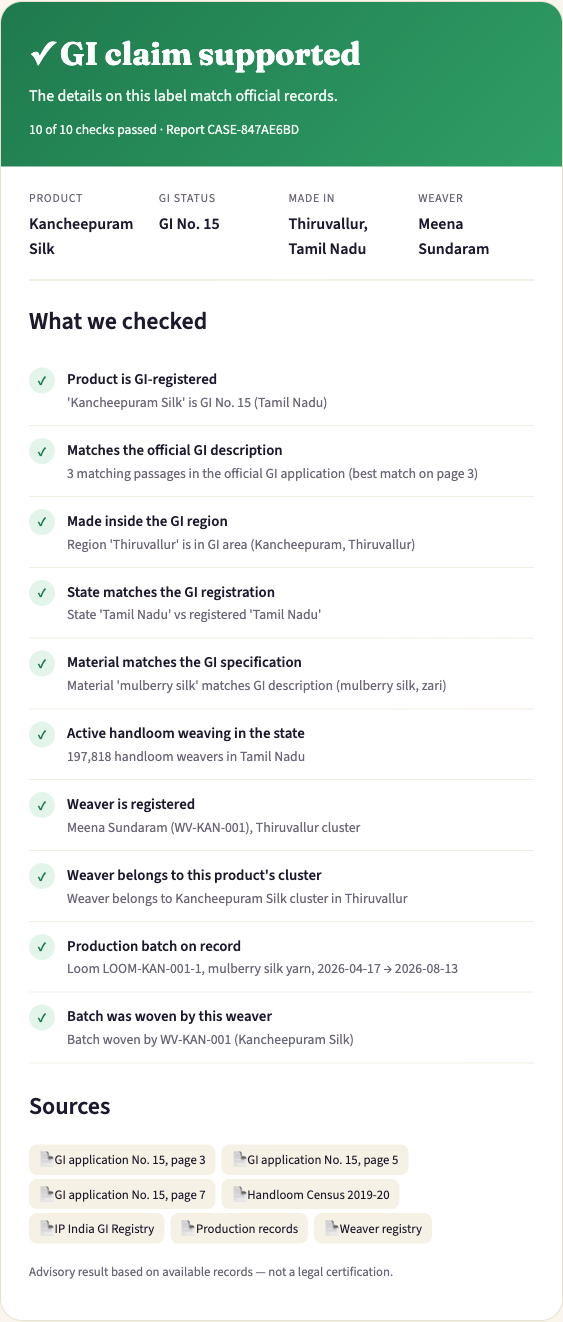
\includegraphics[width=\linewidth,height=8.5cm,keepaspectratio]{figures/ui_supported.png}\\[2pt]
{\footnotesize (a) Supported (alias resolved)}
\end{minipage}\hfill
\begin{minipage}[t]{0.48\linewidth}\centering
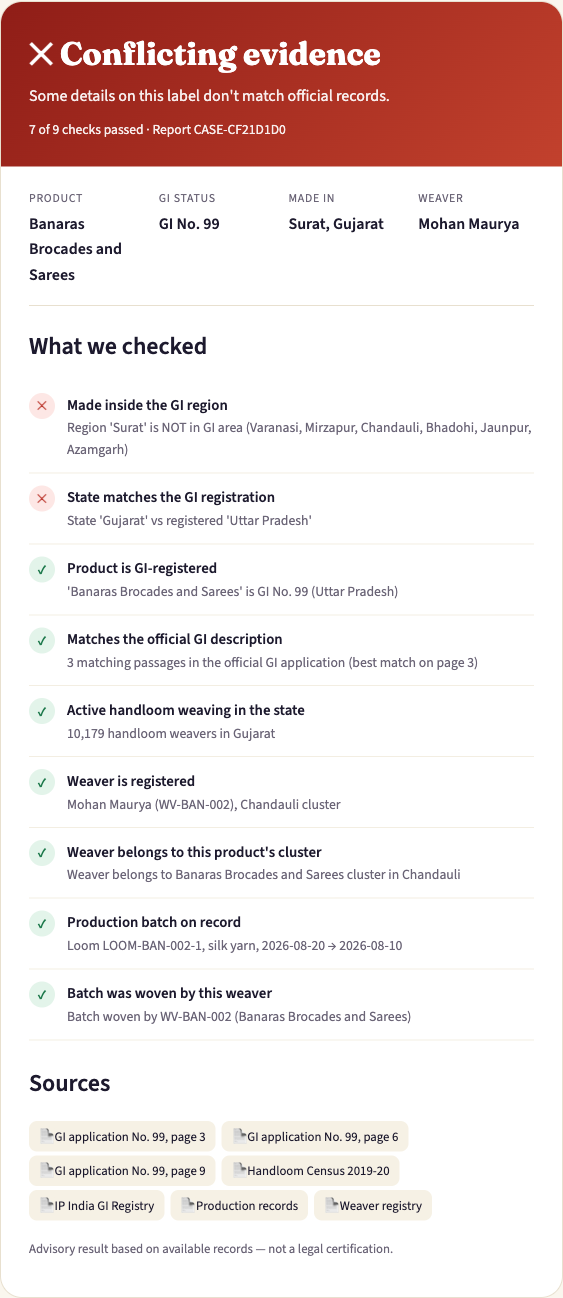
\includegraphics[width=\linewidth,height=8.5cm,keepaspectratio]{figures/ui_conflicting.png}\\[2pt]
{\footnotesize (b) Conflicting evidence (wrong region)}
\end{minipage}
\caption{Verification reports produced by the interface for two claims}
\label{fig:ui}
\end{figure}

\section{Repository Structure}

Listing~\ref{lst:repo} shows the layout of the repository and the purpose of each main file.

\begin{lstlisting}[language={},numbers=none,caption={Repository layout},label={lst:repo}]
loomtrace/
|-- README.md             # setup and run instructions
|-- requirements.txt      # streamlit, langgraph, pydantic, pandas, groq
|-- app.py                # Streamlit website (6 pages)
|-- run_tests.py          # 15 demonstration cases -> TEST_RESULTS.md
|-- loomtrace/
|   |-- agent.py          # CaseState, 6 nodes, graph, guardrail, SLM wrapper, baseline
|   |-- tools.py          # 7 tools, BM25 index, SQLite tables, review helpers
|   |-- data.py           # registry (15 GIs), census (31 rows), passages,
|   |                     #   simulated weaver and batch generator
|   |-- evaluate.py       # 45-case golden set and metrics
|   |-- experiments.py    # repeated evaluation and A/B experiment -> results/
|-- results/experiments.json  # raw numbers used in Chapters 7 and 8
|-- loomtrace.db          # SQLite: checkpoints, cases, review_queue, decisions
\end{lstlisting}
